\documentclass[12pt, a4paper]{article}
% \usepackage{ctex}
\usepackage[margin=1in]{geometry} 
\usepackage{amsmath,amsthm,amssymb}
\usepackage{bm}
\usepackage{cases}
\usepackage{graphicx}
\usepackage{subfig}
\usepackage{hyperref}
\usepackage{amsfonts}
\usepackage{authblk}
\usepackage{mathrsfs}
\newcommand{\E}{\mathbb{E}}
\newcommand{\R}{\mathbb{R}}
\newcommand{\N}{\mathcal{N}}
\hypersetup{hidelinks}
\title{PRML Note\\C09 Mixture Models and EM}
\author{Yang Zhao}
\affil{Department of Automation, Tsinghua University}
\date{}

\begin{document}
    \maketitle
    \section{K-means Clustering}
    \begin{itemize}
        \item Suppose we have a data set $\{\bm{x}_1,\bm{x}_2,\cdots,\bm{x}_N\}$ and 
        our goal is to partition the data set into some number $K$ of clusters, where
        we shall suppose for the moment that the value of $K$ is given.
        \item We might think of a cluster as comprising a group of data points whose
        inter-point distances are small compared with the distances to points outside
        of the cluster. To do this, we introduce a set of D-dimensional vectors 
        $\bm{\mu}_k$, where $k=1,\cdots,K$, in which $\bm{\mu}_k$ is a prototype 
        associated with the $k^{th}$ cluster.
        \item For each data point, we introduce a corresponding set of binary indicator
        variables $r_{nk}\in\{ 0,1\}$, where $k=1,\cdots,K$ describing which of $K$
        clusters the data point $\bm{x}_n$ is designed to, so that if data point 
        $\bm{x}_n$ is designed to cluster $k$, then $r_{nk}=1$ and $r_{nj}=0$ for 
        $j\neq k$. This is known as the $1$-of-$K$ coding scheme. We can define an 
        objective function, sometimes called a \textit{distortion measure}, given by
        \begin{equation}
            J=\sum_{n=1}^N\sum_{k=1}^K r_{nk}\Vert\bm{x}_n-\bm{\mu}_k\Vert^2
        \end{equation}
        Our goal is to find values for the $r_{nk}$ and the $\bm{\mu}_k$ so as to 
        minimize $J$.
        \item First we choose some initial values for the $\bm{\mu}_k$. Then in the 
        first phase we minimize $J$ with respect to the $r_{nk}$, keeping the 
        $\bm{\mu}_k$ fixed. In the second phase we minimize $J$ with respect to the 
        $\bm{\mu}_k$, keeping the $r_{nk}$ fixed. This two-stage optimization is then 
        repeated until convergence. 
        \item Consider first the detemination of the $r_{nk}$. We can simply assign the
        $n^{th}$ data point to the closest cluster centre.
        \begin{equation}
            r_{nk}=\begin{cases}
                1&\textit{if $k=argmin_j\Vert\bm{x}_n-\bm{\mu}_j\Vert^2$}\\
                0&\textit{otherwise}
            \end{cases}
        \end{equation}
        \item Consider the optimization of the $\bm{\mu}_k$ with the $r_{nk}$ held fixed.
        The objective function can be minimized by setting its derivative with respect to
        $\bm{\mu}_k$ to zero giving
        \begin{equation}
            \bm{\mu}_k=\frac{\sum_nr_{nk}\bm{x}_n}{\sum_nr_{nk}}
        \end{equation}
        \item This $K$-means algorithm may converge to a local rather than global 
        minimum of $J$.
        \item In practice, a better initialization procedure would be to choose the 
        cluster centres $\bm{\mu}_k$ to be equal to a random subset of $K$ data points.
        \item It is worth noting that the $K$-means algorithm itself is often used to 
        initialize the parameters in a Gaussian mixture model before applying the EM
        algorithm.
        \item The $K$-means algorithm can be generalized by introducing a more general
        dissimilarity measure $\nu(\bm{x},\bm{x}')$ instead of the Euclidean distance, 
        which gives the $K$-medoids algorithm.
    \end{itemize}
    \section{Mixtures of Gaussians}
    \begin{itemize}
        \item The Gaussian mixture distribution can be written as a linear superposition
        of Gaussians in the form
        \begin{equation}
            p(\bm{x})=\sum_{k=1}^K\pi_k\N(\bm{x}|\bm{\mu}_k,\mathbf{\Sigma}_k)
        \end{equation}
        Let us introduce a $K$-dimensional binary random variable $\bm{z}$ to represent 
        the state of the Gaussian distribution using $1$-of-$K$ code. 
        \begin{figure}[htbp]
            \centering
            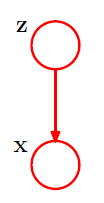
\includegraphics[width=0.75in]{figures/MixtureModel.PNG}
            \caption{Graphical representation of a mixture model}
        \end{figure}
        \item The joint distribution is expressed in the form $p(\bm{x},\bm{z})=p(\bm{z})
        p(\bm{x}|\bm{z})$. The marginal distribution over $\bm{z}$ is specified in terms 
        of the mixing coefficients $\pi_k$, such that
        \begin{equation}
            p(z_k=1)=\pi_k
        \end{equation}
        and the conditional distribution of $\bm{x}$ given a particular value for $\bm{z}$
        is a Gaussian 
        \begin{equation}
            p(\bm{x}|z_k=1)=\N(\bm{x}|\bm{\mu}_k,\mathbf{\Sigma}_k)
        \end{equation}
        So the joint distribution is given by
        \begin{equation}
            p(\bm{x})=\sum_{k=1}^K\pi_k\N(\bm{x}|\bm{\mu}_k,\mathbf{\Sigma}_k)
        \end{equation}
        \item We use $\gamma(z_k)$ to denote $p(z_k=1|\bm{x})$, whose value can be found
        using Bayes' theorem
        \begin{equation}
            \label{eq:responsibility}
            \gamma(z_k)\equiv p(z_k=1|\bm{x})=\frac{\pi_k\N(\bm{x}|\bm{\mu}_k,
            \mathbf{\Sigma}_k)}{\sum_{j=1}^K\pi_j\N(\bm{x}|\bm{\mu}_j,\mathbf{\Sigma}_j)}
        \end{equation}
        the $\gamma(z_k)$ can be viewed as the \textit{responsibility} that component $k$
        takes for explaining the observation $\bm{x}$. $\gamma(z_{nk})\equiv 
        p(z_k=1|\bm{x}_n)$.
        \item Suppose we have a data set of observations $\{\bm{x}_1,\cdots,\bm{x}_N\}$. 
        The log of the likelihood function is given by
        \begin{equation}
            \label{eq:MLEforGM}
            lnp(\mathbf{X}|\bm{\pi},\bm{\mu},\mathbf{\Sigma})=\sum_{n=1}^Nln
            \Big\{\sum_{k=1}^K\pi_k\N(\bm{x}_n|\bm{\mu}_k,\mathbf{\Sigma}_k)\Big\}
        \end{equation}
        It is worth emphasizing that there is a significant problem associated with the 
        maximum likelihood framework applied to Gaussian mixture models, due to the 
        presence of singularities. 
        \item These singularities provide another example of the severe over-fitting that
        can occur in a maximum likelihood approach. If we adopt a Bayesian approach, this
        difficulty does not occur. 
        \item \textit{EM algorithm}. The expectation-maximization algorithm is an elegant
        and powerful method for finding maximum likelihood solutions for models with 
        latent variables. The EM algorithm can be generalized to obtain the variational
        inference framework. 
        \item Setting the derivatives of $lnp(\mathbf{X}|\bm{\pi},\bm{\mu},
        \mathbf{\Sigma})$ in equation (\ref{eq:MLEforGM}) with respect to the $\bm{\mu}_k$
        and $\mathbf{\Sigma}_k$ to zero, we obtain
        \begin{align}
            \label{eq:mean}
            \bm{\mu}_k&=\frac{1}{N_k}\sum_{n=1}^N\gamma(z_{nk})\bm{x}_n\\
            \label{eq:corvariance}
            \mathbf{\Sigma}_k&=\frac{1}{N_k}\sum_{n=1}^N\gamma(z_{nk})
            (\bm{x}_n-\bm{\mu}_k)(\bm{x}_n-\bm{\mu}_k)^T
        \end{align}
        where we have defined
        \begin{equation}
            N_k=\sum_{n=1}^N\gamma(z_{nk})
        \end{equation}
        \item If we want to maximize $lnp(\mathbf{X}|\bm{\pi},\bm{\mu},\mathbf{\Sigma})$
        with respect to the $\pi_k$, we must take account of the constriant $\sum_{k=1}
        ^K\pi_k=1$. This can be achieved using a Lagrange multiplier and maximize the 
        following quantity
        \begin{equation}
            lnp(\mathbf{X}|\bm{\pi},\bm{\mu},\mathbf{\Sigma})+\lambda\Big(
                \sum_{k=1}^K\pi_k-1\Big)
        \end{equation}
        which gives
        \begin{equation}
            0=\sum_{n=1}^N\frac{\N(\bm{x}_n|\bm{\mu}_k,\mathbf{\Sigma}_k)}
            {\sum_j\pi_j\N(\bm{x}_n|\bm{\mu}_j,\mathbf{\Sigma}_j)}+\lambda
        \end{equation}
        If we multiply both sides by $\pi_k$ and sum over $k$ making use of the 
        constriant $\sum_{k=1}^K\pi_k=1$, we can find $\lambda=-N$ and we can obtain
        \begin{equation}
            \label{eq:coefficient}
            \pi_k=\frac{N_k}{N}
        \end{equation}
        \item For EM algorithm, in the expectation step, or E step, we use the current
        values for the parameters to evaluate the posterior probabilities, or 
        responsibility given by equation (\ref{eq:responsibility}); in the maximization
        step, or M step, we use the probabilities to re-estimate the means, corvariances
        and mixing coefficients using the equation (\ref{eq:mean}), 
        (\ref{eq:corvariance}), (\ref{eq:coefficient}). 
    \end{itemize}
    \section{An Alternative View of EM}
    \begin{itemize}
        \item The goal of the EM algorithm is to find maximum likelihood solutions for 
        models having latent variables. We denote the set of all observed data by 
        $\mathbf{X}$, in which the $n^{th}$ row represents $\bm{x}_n^T$, and similarly
        we denote the set of all latent variables by $\mathbf{Z}$, with a corresponding
        row $\bm{z}_n^T$. The set of all model parameters is denoted by $\bm{\theta}$, 
        and so the log likelihood function is given by
        \begin{equation}
            ln p(\mathbf{X}|\bm{\theta})=ln\Big\{\sum_{\mathbf{Z}}p(\mathbf{X},
            \mathbf{Z}|\bm{\theta}) \Big\}
        \end{equation}
        \item The presence of the sum prevents the logarithm from acting directly on the 
        joint distribution, resulting in complicated expressions for the maximum likelihood
        solution. 
        \item \textit{The General EM Algorithm}. \begin{enumerate}
            \item Choose an initial setting for the parameters $\bm{\theta}^{old}$.
            \item \textbf{E Step}. Evaluate $p(\mathbf{Z}|\mathbf{X},\bm{\theta}^{old})$.
            \item \textbf{M Step}. Evaluate $\bm{\theta}^{new}$ given by 
            \begin{equation*}
                \bm{\theta}^{new}=argmax_{\bm{\theta}} Q(\bm{\theta},\bm{\theta}^{old})
            \end{equation*}
            where \begin{equation*}
                Q(\bm{\theta},\bm{\theta}^{old})=\sum_{\mathbf{Z}}p(\mathbf{Z}|\mathbf{X},
                \bm{\theta}^{old})ln p(\mathbf{X},\mathbf{Z}|\bm{\theta})
            \end{equation*}
            \item Check for convergence of either the log likelihood or the parameters values.
            If the convergence criterion is not satisfied, then let
            \begin{equation*}
                \bm{\theta}^{old}\leftarrow\bm{\theta}^{new}
            \end{equation*}
            and return to step 2. 
        \end{enumerate}
        \item The EM algorithm can also be used to find MAP solutions for models in which a 
        prior $p(\bm{\theta})$ is defined over the parameters. In this case the E step remains
        the same as in the maximum likelihood case, whereas in the M step the quantity to be 
        maximized is given by $Q(\bm{\theta},\bm{\theta}^{old})+lnp(\bm{\theta})$. Suitable 
        choices for the prior will remove the singularities. 
    \end{itemize}
\end{document}
